\begin{frame}{Electronic Design Automation (EDA) : }

  \begin{columns}[T]

    \begin{column}{0.52\textwidth}
      \begin{itemize}
        \setlength{\itemsep}{4pt}
        \item \textbf{Spécification système} : besoins et fonctionnalités
        \item \textbf{Conception architecturale} : partitionnement HW/SW
        \item \textbf{Conception fonctionnelle et RTL} : description HDL (Verilog/VHDL)
        \item \textbf{Synthèse logique} : RTL $\rightarrow$ netlist de portes
        \item \textbf{Conception physique} : placement et routage
        \item \textbf{Vérification physique et signoff} : DRC, LVS, STA
        \item \textbf{Fabrication} : gravure sur wafer (silicium)
        \item \textbf{Packaging et test} : mise en boîtier, tests
        \item \textbf{Puce finale} : circuit intégré prêt à l'emploi
      \end{itemize}
    \end{column}


    \begin{column}{0.44\textwidth}
      \centering
      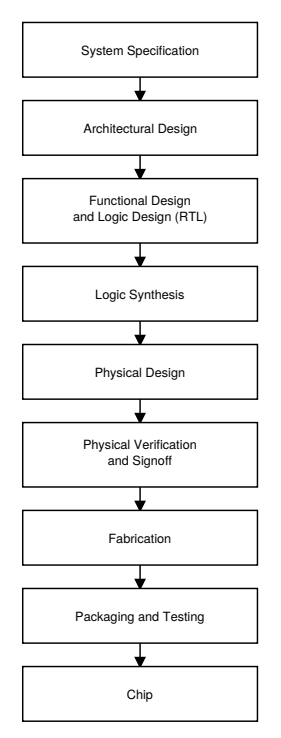
\includegraphics[width=\textwidth,height=0.85\textheight,keepaspectratio]{./images/eda_flow.png}
      %\includesvg[width=\textwidth,height=0.85\textheight,keepaspectratio]{./images/eda_flow.svg}
    \end{column}

  \end{columns}
\end{frame}
